\documentclass{beamer}
%\usepackage{xspace}
\usepackage{amsmath,amssymb}
\usepackage{graphicx}
%\usepackage{svg}
%\usepackage{pgfpages}
%\pgfpagesuselayout{4 on 1}[a4paper,border shrink=5mm,landscape]
%\usepackage{psfrag}
%\usepackage[usenames,dvipsnames]{xcolor}
\usepackage{braket}
\usepackage{tikz}
\usetikzlibrary{graphs}
\usetikzlibrary{datavisualization}
\usetikzlibrary{datavisualization.formats.functions}
\usepackage{pgfplotstable}
\usepgfplotslibrary{patchplots}

\setbeamercovered{transparent}

\usetheme{Pittsburgh}
%\usetheme{default}

\setbeamertemplate{sidebar right}{}
\setbeamertemplate{footline}[frame number]
%\usefonttheme{professionalfonts}

%\usepackage{sansmathaccent}
%\usepackage{bm}

%\usepackage{unicode-math}
%%\setmainfont[SlantedFont={Latin Modern Roman Slanted},SlantedFeatures={Color=000000},
%%  SmallCapsFont={TeX Gyre Termes},SmallCapsFeatures={Letters=SmallCaps}]{XITS}
%\setmathfont[math-style=ISO,sans-style=upright]{XITS Math}
%\setmathfont[range={\mathcal,\mathbfcal}]{Latin Modern Math}

\usepackage{sfmath}

%\mathversion{sans}

\newcommand{\Tr}{\mathsf{Tr}}

\definecolor{redorange}{rgb}{1.0, .25, .25}
\definecolor{citation}{rgb}{.1, 0.8, .35}
\newcommand\emm[1]{\textcolor{redorange}{{#1}}}
\newcommand\numc[1]{\textcolor{citation}{{\bf #1}}}

%\newcommand\bm[1]{{\mbox{\boldmath $#1$}}}
\newcommand\bm[1]{{\mathbf{#1}}}
%\newcommand\bm[1]{{\bf #1}}
%\newcommand\bm[1]{\ensuremath{\boldsymbol{#1}}}
%\newcommand\bm[1]{{\textbf{\it #1}}}

\title{Nonlocality and Tsirelson's bound}
\author{Ryuhei Mori}
%\institute{$\vcenter{\hbox{\includegraphics[width=30pt]{ELC_logo}}}$ Postdoctoral Fellow of ELC\\ $\vcenter{\hbox{\includegraphics[width=20pt]{titech_logo}}}$ Tokyo Institute of Technology}
\institute{Tokyo Institute of Technology}
\date{23, Oct., 2020}



\begin{document}
\begin{frame}[plain]
\maketitle
\end{frame}



\begin{frame}{Bell test: CHSH game (1964, 1969)}
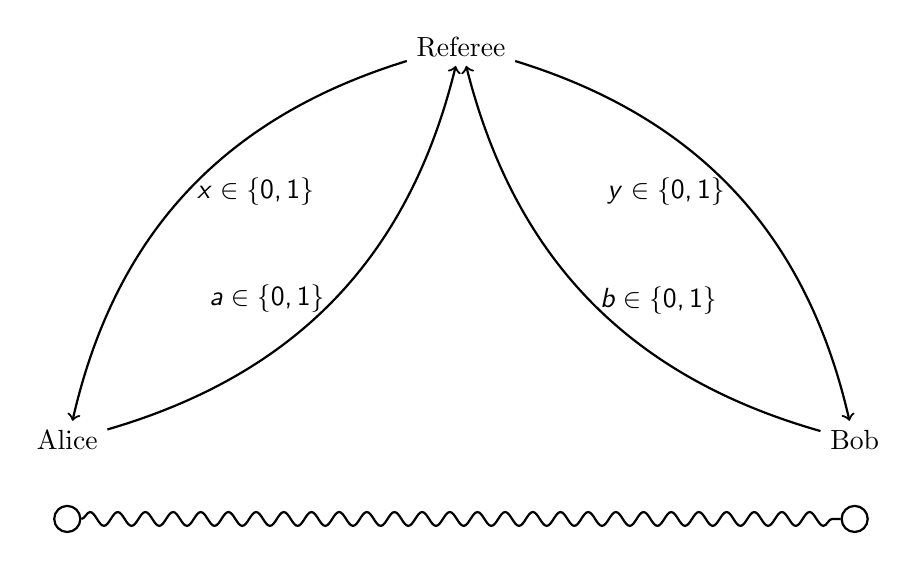
\begin{tikzpicture}
\node at (5,5) (R) {Referee};
\node at (0,0) (A) {Alice};
\node at (10,0) (B) {Bob};
\node at (0,-1)[circle,thick,draw] (As) {};
\node at (10,-1)[circle,thick,draw] (Bs) {};
\draw[->,thick] (R) edge[bend right] node[anchor=west, midway]{$x\in\{0,1\}$} (A);
\draw[->,thick] (R) edge[bend left] node[anchor=east, midway]{$y\in\{0,1\}$} (B);
\draw[->,thick] (A) edge[bend right] node[anchor=east, midway]{$a\in\{0,1\}$} (R);
\draw[->,thick] (B) edge[bend left] node[anchor=west, midway]{$b\in\{0,1\}$} (R);
\draw[thick,decorate,decoration=snake] (As) -- (Bs);
\end{tikzpicture}
%\includegraphics[width=30pt]{Alice_in_Wonderland.png}
\begin{center}
Alice and Bob win iff $\emm{a\oplus b = x\wedge y}$.
\end{center}
\end{frame}

\begin{frame}{Bell inequality}
$a_x$: Output of Alice for given $x$.

$b_y$: Output of Bbob for given $y$.
\begin{align*}
a_0 \oplus b_0 &= 0\\
a_1 \oplus b_0 &= 0\\
a_0 \oplus b_1 &= 0\\
a_1 \oplus b_1 &= 1
\end{align*}
By adding all equations, we get $0=1$, which means there is no solution.
Hence, the winning probability 1 cannot be achieved.

\vspace{1em}
Three equalities can be satisfied, so that the largest winning probability is \emm{3/4}~(Bell inequality or CHSH inequality).

\vspace{1em}
If Alice and Bob share quantum states, then the largest winning probability is
$(2+\sqrt{2})/4\approx \emm{0.854}$~(Violation of Bell/CHSH inequality)
\end{frame}

\begin{frame}{Locality (Hidden variable model)}
\begin{center}
Joint preparation and independent measurements.
\end{center}
Probability distribution $P(a,b\mid x,y)$ is said to be \emm{local} if
\begin{equation*}
P(a, b\mid x,y) = \sum_{\lambda} P(\lambda) P(a\mid x, \lambda) P(b\mid y,\lambda).
\end{equation*}
\vspace{2em}
\begin{center}
Quantum physics allow \emm{nonlocal} behaviors.
\end{center}
\end{frame}

\begin{frame}{Joint probability distribuion}
\small
\begin{lemma}
There exists probability distributions $P(\lambda)$, $P(a\mid x,\lambda)$ and $P(b\mid y,\lambda)$ such that
\begin{equation*}
P(a, b\mid x,y) = \sum_{\lambda} P(\lambda) P(a\mid x, \lambda) P(b\mid y,\lambda)
\end{equation*}
if and only if there exists probability distribution $q(a_0,a_1,b_0,b_1)$ such that
\begin{equation*}
P(a, b\mid x,y) = \sum_{\substack{a_0,a_1,b_0,b_1\\a_x = a,\, b_y = b}} q(a_0, a_1, b_0, b_1).
\end{equation*}
\end{lemma}

\vspace{-2em}
\begin{proof}
\begin{align*}
(\Rightarrow)\qquad
q(a_0,a_1,b_0,b_1) &:= \sum_{\lambda}P(\lambda) P(a_0\mid x=0, \lambda) P(a_1\mid x=1, \lambda)\\
&\cdot P(b_0\mid y=0, \lambda) P(b_1\mid y=1, \lambda)
\end{align*}
\begin{equation*}
(\Leftarrow)\qquad
\lambda = (a_0, a_1, b_0, b_1), \qquad P(\lambda) = q(a_0,a_1,b_0,b_1)
%P(a, b\mid x,y) = \sum_{\lambda} P(\lambda) P(a\mid x, \lambda) P(b\mid y,\lambda).
\end{equation*}
\end{proof}
\end{frame}

\begin{frame}{Randomness doesn't help}
\begin{align*}
\mathbb{E}_{x,y}\left[\mathbb{E}_{a_0,a_1,b_0,b_1}\left[\mathbb{I}\{a_x\oplus b_y = x\wedge y\}\right]\right]\\
=
\mathbb{E}_{a_0,a_1,b_0,b_1}\left[\mathbb{E}_{x,y}\left[\mathbb{I}\{a_x\oplus b_y = x\wedge y\}\right]\right].
\end{align*}

\vspace{2em}
There exists $a^*_0,a^*_1,b^*_0,b^*_1$ such that
\begin{align*}
\mathbb{E}_{a_0,a_1,b_0,b_1}\left[\mathbb{E}_{x,y}\left[\mathbb{I}\{a_x\oplus b_y = x\wedge y\}\right]\right]
\le
\mathbb{E}_{x,y}\left[\mathbb{I}\{a^*_x\oplus b^*_y = x\wedge y\}\right].
\end{align*}
\end{frame}

\begin{frame}{Einstein--Podolsky--Rosen (EPR) paradox (1935)}
\begin{equation*}
P(a, b\mid x,y) = \sum_{\lambda} P(\lambda) P(a\mid x, \lambda) P(b\mid y,\lambda).
\end{equation*}
$\iff$
there exists a joint distribution of $(a_0,a_1,b_0,b_1)$.

\begin{center}
\Large
$\Downarrow$

\vspace{1.0em}
\normalsize
In quantum physics,
$a_0,a_1,b_0,b_1$ \emm{cannot \textit{exists}} simultaneously.

\vspace{1.0em}
\Large
$\Downarrow$

\vspace{1.0em}
\normalsize
In quantum physics,
position and momentum \emm{cannot \textit{exists}} simultaneously.
\end{center}

%[Einstein, Podolsky, Rosen 1935, \numc{15771}]
\end{frame}

\if0
\begin{frame}{Bell state}
\small
\begin{lemma}
For any orthonormal basis $\{\ket{\psi_0},\,\ket{\psi_1}\}$ of $\mathbb{C}^2$,
\begin{equation*}
\frac1{\sqrt{2}}(\ket{0}\ket{0} + \ket{1}\ket{1})
=
\frac1{\sqrt{2}}(\ket{\psi_0}\ket{\psi_0}^* + \ket{\psi_1}\ket{\psi_1}^*).
\end{equation*}
\end{lemma}

\vspace{-1em}
\begin{proof}
There exist $\theta,\,\eta\in\mathbb{R}$ and $\alpha,\,\beta\in\mathbb{C}$ satisfying $|\alpha|^2+|\beta|^2=1$ such that
\begin{align*}
\ket{\psi_0} &:= \mathsf{e}^{i\theta}(\alpha \ket{0} + \beta \ket{1})\\
\ket{\psi_1} &:= \mathsf{e}^{i\eta}(\beta^* \ket{0} - \alpha^* \ket{1}).
\end{align*}

\vspace{-2.5em}
\begin{align*}
&\frac1{\sqrt{2}}(\ket{\psi_0}\ket{\psi_0}^* + \ket{\psi_1}\ket{\psi_1}^*)\\
&= \frac1{\sqrt{2}}(|\alpha|^2\ket{0}\ket{0} + \alpha\beta^*\ket{0}\ket{1} + \beta\alpha^*\ket{1}\ket{0} + |\beta|^2\ket{1}\ket{1}\\
&\qquad + |\beta|^2\ket{0}\ket{0} - \beta^*\alpha\ket{0}\ket{1} - \alpha^*\beta\ket{1}\ket{0} + |\alpha|^2\ket{1}\ket{1})\\
&= \frac1{\sqrt{2}}(\ket{0}\ket{0} + \ket{1}\ket{1}).
\end{align*}
\end{proof}
\end{frame}
\fi


\begin{frame}{Bell state}
\small

%For $\ket{\psi_\theta} := \cos\theta\ket{0}+\sin\theta\ket{1}$.
Bell state
\begin{equation*}
\ket{\Psi}:=
\frac1{\sqrt{2}}(\ket{0}\ket{0} + \ket{1}\ket{1})
%=
%\frac1{\sqrt{2}}(\ket{\psi_\theta}\ket{\psi_\theta} + \ket{\psi_{\theta+\pi/2}}\ket{\psi_{\theta+\pi/2}}).
\end{equation*}

\vspace{2em}
Let $\ket{\psi_\theta} := \cos\theta\ket{0}+\sin\theta\ket{1}$.

Alice measure this state by $\{\ket{\psi_{\theta_A}}, \ket{\psi_{\theta_A+\pi/2}}\}$.

Bob measure this state by $\{\ket{\psi_{\theta_B}}, \ket{\psi_{\theta_B+\pi/2}}\}$.

\vspace{1.5em}
A outcome corresponding to $\ket{\psi_\theta}\ket{\psi_\tau}$ is obtained with probability
\begin{align*}
|\bra{\psi_{\theta}}\bra{\psi_{\tau}}\ket{\Psi}|^2
&=\Bigl|\bra{\psi_{\theta}}\bra{\psi_{\tau}}
\frac1{\sqrt{2}}(\ket{0}\ket{0} + \ket{1}\ket{1})\Bigr|^2\\
%&=\frac12 |\braket{\psi_\tau\mid \psi_\theta}|^2\\
&=\frac12 |\cos\theta\cos\tau + \sin\theta\sin\tau|^2
=\emm{\frac12 \cos^2(\theta-\tau)}.
\end{align*}
Another proof:
\begin{align*}
\bra{\psi_{\theta}}\bra{\psi_{\tau}}\ket{\Psi}
&= \Tr\left(\mathcal{M}(\ket{\psi_\theta}\ket{\psi_\tau})^\dagger\mathcal{M}(\ket{\Psi})\right)\\
&= \Tr\left(\ket{\psi_\tau}\bra{\psi_\theta}\frac1{\sqrt{2}} I\right)
= \frac1{\sqrt{2}} \braket{\psi_\theta|\psi_\tau}
\end{align*}
\end{frame}

\begin{frame}{Quantum strategy}
\begin{center}
\begin{tikzpicture}
\draw[->,thick] (0,0) to (2,0);
\draw[->,thick] (0,0) to (0,2);
\draw[->,dashed,thick] (0,0) to ({2*cos(45)},{2*sin(45)});
\draw[->,dashed,thick] (0,0) to ({2*cos(135)},{2*sin(135)});;
\draw[->,thick] (5,0) to ({5+2*cos(22.5)},{2*sin(22.5)});
\draw[->,thick] (5,0) to ({5+2*cos(112.5)},{2*sin(112.5)});
\draw[->,dashed,thick] (5,0) to ({5+2*cos(-22.5)},{2*sin(-22.5)});
\draw[->,dashed,thick] (5,0) to ({5+2*cos(67.5)},{2*sin(67.5)});;
\end{tikzpicture}
\end{center}
\begin{align*}
\theta_A^{x=0} &= 0, & \theta_A^{x=1} &= \pi/4, &
\theta_B^{y=0} &= \pi/8, & \theta_B^{y=1} &= -\pi/8
\end{align*}
For any $x\in\{0,1\}, y\in\{0,1\}$, the winning probability is
\begin{equation*}
\cos^2\left(\frac{\pi}8\right)
=
\frac{2+\sqrt{2}}4
\approx 0.854.
\end{equation*}
\end{frame}

\begin{frame}{XOR game}
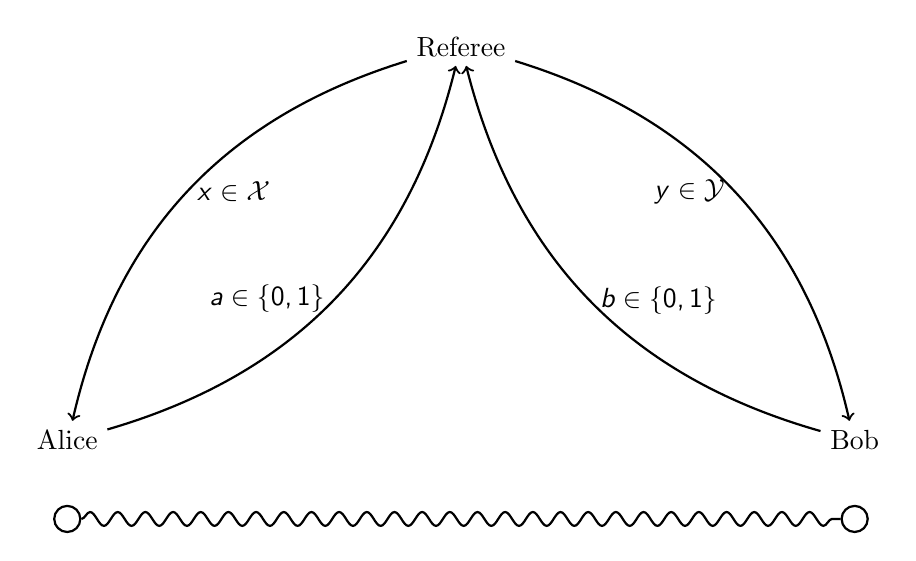
\begin{tikzpicture}
\node at (5,5) (R) {Referee};
\node at (0,0) (A) {Alice};
\node at (10,0) (B) {Bob};
\node at (0,-1)[circle,thick,draw] (As) {};
\node at (10,-1)[circle,thick,draw] (Bs) {};
\draw[->,thick] (R) edge[bend right] node[anchor=west, midway]{$x\in\mathcal{X}$} (A);
\draw[->,thick] (R) edge[bend left] node[anchor=east, midway]{$y\in\mathcal{Y}$} (B);
\draw[->,thick] (A) edge[bend right] node[anchor=east, midway]{$a\in\{0,1\}$} (R);
\draw[->,thick] (B) edge[bend left] node[anchor=west, midway]{$b\in\{0,1\}$} (R);
\draw[thick,decorate,decoration=snake] (As) -- (Bs);
\end{tikzpicture}
%\includegraphics[width=30pt]{Alice_in_Wonderland.png}
\begin{center}
Alice and Bob win iff $\emm{a\oplus b = f(x, y)}$.
\end{center}
\end{frame}


\begin{frame}{Tsirelson's theorem}
The maximum quantum winning probability is
\begin{align*}
\max\colon\qquad& \sum_{x,y}p(x,y)\sum_{\substack{a,b\\ a\oplus b = f(x,y)}} \Tr(\rho (P_a^{(x)} \otimes Q_b^{(y)}))\\
\text{subject to}\colon\qquad&
n\in\mathbb{N}\\
&\rho \in \mathcal{H}(\mathbb{C}^n\otimes\mathbb{C}^n)\\
&\rho\succeq 0\\
&\Tr(\rho) = 1\\
&P_a^{(x)},\, Q_b^{(y)} \in \mathcal{H}(\mathbb{C}^n)\qquad  \forall x,y,a,b\\
&P_a^{(x)} \succeq 0\qquad \forall x, a \\
&Q_b^{(y)} \succeq 0\qquad \forall y, b \\
&P_0^{(x)} + P_1^{(x)} = I\qquad \forall x\\
&Q_0^{(y)} + Q_1^{(y)} = I\qquad \forall y.
\end{align*}
\end{frame}

\begin{frame}{Tsirelson's theorem}
The maximum quantum winning probability is
\begin{align*}
\max\colon\qquad& \sum_{x,y}p(x,y)\sum_{\substack{a,b\\ a\oplus b = f(x,y)}} \emm{\bra{\psi}}P_a^{(x)} \otimes Q_b^{(y)}\emm{\ket{\psi}}\\
\text{subject to}\colon\qquad&
n\in\mathbb{N}\\
&\emm{\ket{\psi}} \in \mathbb{C}^n\otimes\mathbb{C}^n\\
&\emm{\braket{\psi|\psi}}=1\\
&P_a^{(x)},\, Q_b^{(y)} \in \mathcal{H}(\mathbb{C}^n)\qquad  \forall x,y,a,b\\
&P_a^{(x)} \succeq 0\qquad \forall x, a \\
&Q_b^{(y)} \succeq 0\qquad \forall y, b \\
&P_0^{(x)} + P_1^{(x)} = I\qquad \forall x\\
&Q_0^{(y)} + Q_1^{(y)} = I\qquad \forall y.
\end{align*}
\end{frame}

\begin{frame}{Binary measurements}
\begin{lemma}
\begin{align*}
P_0\succeq 0,\, P_1\succeq 0,\, P_0+P_1=I
\iff
\exists P,\, I - P^2 \succeq 0, 
P_a = \frac{I+(-1)^aP}2.
\end{align*}
\end{lemma}
\begin{proof}
$(\Rightarrow)$ $P=P_0-P_1$.

\vspace{1em}
$(\Leftarrow)$ 
\begin{align*}
\frac{I+(-1)^aP}2&\succeq 0\\
\frac{I+P}2 + \frac{I-P}2 &= I.
\end{align*}
\end{proof}
\end{frame}

\begin{frame}{Tsirelson's theorem}
\small
By letting $P^{(x)} := P_0^{(x)} - P_1^{(x)}$ and $Q^{(y)} := Q_0^{(y)} - Q_1^{(y)}$,
the maximum quantum winning probability is
\begin{align*}
\max\colon\qquad& \sum_{x,y}p(x,y)\sum_{\substack{a,b\\ a\oplus b = f(x,y)}} \bra{\psi}\frac{I+(-1)^aP^{(x)}}2\otimes \frac{I+(-1)^b Q^{(y)}}2\ket{\psi}\\
\text{subject to}\colon\qquad&
n\in\mathbb{N}\\
&\ket{\psi} \in \mathbb{C}^n\otimes\mathbb{C}^n\\
&\braket{\psi|\psi}=1\\
&\emm{P^{(x)},\, Q^{(y)}} \in \mathcal{H}(\mathbb{C}^n)\qquad  \forall x,y\\
&I-(P^{(x)})^2\succeq 0\qquad \forall x\\
&I-(Q^{(y)})^2\succeq 0\qquad \forall y\\
%&P_a^x \succeq 0\qquad \forall x, a \in\{0,1\}\\
%&Q_b^{(y)} \succeq 0\qquad \forall y, b \in\{0,1\}\\
%&P_0^x + P_1^x = I\qquad \forall x\in\{0,1\}\\
%&Q_0^y + Q_1^y = I\qquad \forall y\in\{0,1\}.
\end{align*}
\end{frame}

\begin{frame}{Tsirelson's theorem}
\small
The maximum quantum winning probability is
\begin{align*}
\max\colon\,& \sum_{x,y,a,b}p(x,y) \bra{\psi}\frac{I+(-1)^aP^{(x)}}2\otimes\frac{I+(-1)^b Q^{(y)}}2\ket{\psi}\emm{\frac{1+(-1)^{a+b+f(x,y)}}2}\\
\text{s.t.}\colon\,&
n\in\mathbb{N}\\
&\ket{\psi} \in \mathbb{C}^n\otimes\mathbb{C}^n\\
&\braket{\psi|\psi}=1\\
&P^{(x)},\, Q^{(y)} \in \mathcal{H}(\mathbb{C}^n)\qquad  \forall x,y\\
&I-(P^{(x)})^2\succeq 0\qquad \forall x\\
&I-(Q^{(y)})^2\succeq 0\qquad \forall y\\
%&P_a^x \succeq 0\qquad \forall x, a \in\{0,1\}\\
%&Q_b^{(y)} \succeq 0\qquad \forall y, b \in\{0,1\}\\
%&P_0^x + P_1^x = I\qquad \forall x\in\{0,1\}\\
%&Q_0^y + Q_1^y = I\qquad \forall y\in\{0,1\}.
\end{align*}
\end{frame}

\begin{frame}{Tsirelson's theorem}
\small
The maximum quantum winning probability is
\begin{align*}
\max\colon\qquad& \frac12\left(1 + \sum_{x,y}p(x,y) \bra{\psi}P^{(x)}\otimes Q^{(y)}\ket{\psi}(-1)^{f(x,y)}\right)\\
\text{subject to}\colon\qquad&
n\in\mathbb{N}\\
&\ket{\psi} \in \mathbb{C}^n\otimes\mathbb{C}^n\\
&\braket{\psi|\psi}=1\\
&P^{(x)},\, Q^{(y)} \in \mathcal{H}(\mathbb{C}^n)\qquad  \forall x,y\\
&I-(P^{(x)})^2\succeq 0\qquad \forall x\\
&I-(Q^{(y)})^2\succeq 0\qquad \forall y\\
%&P_a^x \succeq 0\qquad \forall x, a \in\{0,1\}\\
%&Q_b^{(y)} \succeq 0\qquad \forall y, b \in\{0,1\}\\
%&P_0^x + P_1^x = I\qquad \forall x\in\{0,1\}\\
%&Q_0^y + Q_1^y = I\qquad \forall y\in\{0,1\}.
\end{align*}
\end{frame}

\begin{frame}{Convexity and extremal points}
\begin{lemma}
A set
\begin{align*}
C:=\left\{P\in \mathcal{H}(\mathbb{C}^n)\mid I-P^2 \succeq 0\right\}
\end{align*}
is a convex set. $P\in C$ is \emm{extremal} if and only if \emm{$P^2=I$}.
\end{lemma}
\begin{proof}
If $P$ has an eigenvalue in $(-1,+1)$, $P$ can be represented by convex combination of two different points in $C$.

\vspace{1em}
Assume $P$ has an eigenvalue in $\pm1$. Let $\ket{\psi}$ be an eigenvector of $P$ for an eigenvalue $\lambda\in\{-1,+1\}$.
If $P=p P_0 + (1-p) P_1$ for some $p\in(0,1)$, $p\bra{\psi}P_0\ket{\psi}+(1-p)\bra{\psi}P_1\ket{\psi}=\lambda$.
This means that $\bra{\psi}P_0\ket{\psi}=\bra{\psi}P_1\ket{\psi}=\lambda$. Hence, $\ket{\psi}$ is also an eigenvector of $P_0$ and $P_1$.
All eigenvectors of $P$ are also eigenvectors of $P_0$ and $P_1$ for the same eigenvalue. Hence, $P_0=P_1=P$.
\end{proof}
\end{frame}

\begin{frame}{Tsirelson's theorem}
\small
The maximum quantum winning probability is
\begin{align*}
\max\colon\qquad& \frac12\left(1 + \sum_{x,y}p(x,y) \bra{\psi}P^{(x)}\otimes Q^{(y)}\ket{\psi}(-1)^{f(x,y)}\right)\\
\text{subject to}\colon\qquad&
n\in\mathbb{N}\\
&\ket{\psi} \in \mathbb{C}^n\otimes\mathbb{C}^n\\
&\braket{\psi|\psi}=1\\
&P^{(x)},\, Q^{(y)} \in \mathcal{H}(\mathbb{C}^n)\qquad  \forall x,y\\
&(P^{(x)})^2\,\emm{=}\,I\qquad \forall x\\
&(Q^{(y)})^2\,\emm{=}\,I\qquad \forall y
\end{align*}
Here, $P^{(x)}$ and $Q^{(y)}$ are \emm{unitary}.
Let 
\begin{align*}
\ket{A_x}&:=(P^{(x)}\otimes I)\ket{\psi}\\
\ket{B_y}&:=(I\otimes Q^{(y)})\ket{\psi}.
\end{align*}
Then, $\bra{\psi}P^{(x)}\otimes Q^{(y)}\ket{\psi} = \braket{A_x|B_y}$.
\end{frame}

\begin{frame}{Tsirelson's theorem}
\small
The maximum quantum winning probability is \emm{at most (in fact, equal to)}
\begin{align*}
\max\colon\qquad& \frac12\left(1 + \sum_{x,y}p(x,y) \emm{\mathsf{Re}\left(\braket{A_x|B_y}\right)} (-1)^{f(x,y)}\right)\\
\text{subject to}\colon\qquad&
n\in\mathbb{N}\\
&\ket{A_x}, \ket{B_y} \in \mathbb{C}^n\otimes\mathbb{C}^n\qquad \forall x,y\\
&\braket{A_x|A_x}=1\qquad\forall x\\
&\braket{B_y|B_y}=1\qquad\forall y
\end{align*}
\end{frame}

\begin{frame}{Real vectors}
%\begin{align*}
%\ket{A_x}&:=(P^{(x)}\otimes I)\ket{\psi}\\
%\ket{B_y}&:=(I\otimes Q^{(y)})\ket{\psi}.
%\end{align*}
For some orthonormal basis $\{\ket{e_i}\}$,
$\ket{A_x}=\sum_{i=1}^{n^2} \alpha_i^{(x)}\ket{e_i}$,
$\ket{B_y}=\sum_{i=1}^{n^2} \beta_i^{(y)}\ket{e_i}$.
Let
\begin{align*}
v_x &:= \begin{bmatrix}\mathsf{Re}(\alpha_1^{(x)})& \mathsf{Im}(\alpha_1^{(x)}) &\mathsf{Re}(\alpha_2^{(x)})&\dotsm&\mathsf{Im}(\alpha_{n^2}^{(x)})\end{bmatrix}\in\mathbb{R}^{2n^2}\\
w_y &:= \begin{bmatrix}\mathsf{Re}(\beta_1^{(y)})& \mathsf{Im}(\beta_1^{(y)}) &\mathsf{Re}(\beta_2^{(y)})&\dotsm&\mathsf{Im}(\beta_{n^2}^{(y)})\end{bmatrix}\in\mathbb{R}^{2n^2}
\end{align*}
Then, $\langle v_x, v_x\rangle = \braket{A_x|A_x}$, $\langle v_x, w_y\rangle = \mathsf{Re}(\braket{A_x|B_y})$.
\end{frame}

\begin{frame}{Tsirelson's theorem [Tsirelson 1980]}
\small
The maximum quantum winning probability is \emm{at most (in fact, equal to)}
\begin{align*}
\max\colon\qquad& \frac12\left(1 + \sum_{x,y}p(x,y) \langle v_x, w_y\rangle(-1)^{f(x,y)}\right)\\
\text{subject to}\colon\qquad&
n\in\mathbb{N}\\
&v_x \in \mathbb{R}^{2n^2}\qquad \forall x\\
&w_y \in \mathbb{R}^{2n^2}\qquad \forall y\\
&\|v_x\| = 1\qquad \forall x\\
&\|w_y\| = 1\qquad \forall y
%&P^{(x)},\, Q^{(y)} \in \mathcal{H}(\mathbb{C}^n)\qquad  \forall x,y\in\{0,1\}\\
%&(P^{(x)})^2=I\qquad \forall x\in\{0,1\}\\
%&(Q^{(y)})^2=I\qquad \forall y\in\{0,1\}\\
\end{align*}

\vspace{3em}
\centering\Large
Tsirelson's bound
\end{frame}

\begin{frame}{SDP programming for Tsirelson's theorem}
\small
The maximum quantum winning probability is \emm{at most (in fact, equal to)}
\begin{align*}
\max\colon\qquad& \frac12\left(1 + \sum_{x,y}p(x,y) C_{x,y} (-1)^{f(x,y)}\right)\\
\text{subject to}\colon\qquad&
C\succeq 0\\
&C_{z,z} = 1\qquad \forall z\in\mathcal{X}\cup\mathcal{Y}
\end{align*}
\end{frame}

\begin{frame}{Tsirelson's bound [Tsirelson 1980]}
\small
\begin{align*}
\max\colon\qquad& \frac12\left(1 + \frac14\sum_{x,y} \langle v_x, w_y\rangle(-1)^{(x\wedge y)}\right)\\
\end{align*}
\begin{align*}
\frac14\sum_{x,y} \langle v_x, w_y\rangle(-1)^{(x\wedge y)}
&= \frac14\left(\langle v_0, w_0\rangle + \langle v_0, w_1\rangle + \langle v_1, w_0\rangle - \langle v_1, w_1\rangle\right)\\
&= \frac14\left(\langle v_0, w_0 + w_1\rangle + \langle v_1, w_0 - w_1\rangle\right)\\
&\,\emm{\le}\, \frac14\left(\|v_0\|\|w_0 + w_1\| + \| v_1\|\|w_0 - w_1\|\right)\\
&= \frac14\left(\|w_0 + w_1\| + \|w_0 - w_1\|\right)\\
&\,\emm{\le}\, \frac{\sqrt{2}}4\sqrt{\|w_0 + w_1\|^2 + \|w_0 - w_1\|^2}\\
&= \frac{\sqrt{2}}4\sqrt{2\|w_0\|^2 + 2\|w_1\|^2}
=\frac1{\sqrt{2}}
\end{align*}
\end{frame}


%\begin{frame}{No-signaling theory}
%\end{frame}


\begin{frame}{Assignments}
\small
\begin{enumerate}
\setlength{\itemsep}{1em}
\item Let
\begin{align*}
T_{2i-1} &:= \underbrace{I\otimes\dotsm\otimes I}_{i-1}\otimes X\otimes \underbrace{Y\otimes\dotsm\otimes Y}_{d-i}\in\mathcal{H}(\mathbb{C}^{2^{d}})\\
T_{2i} &:= \underbrace{I\otimes\dotsm\otimes I}_{i-1}\otimes Z\otimes \underbrace{Y\otimes\dotsm\otimes Y}_{d-i}\in\mathcal{H}(\mathbb{C}^{2^{d}})
\end{align*}
for $i=1,\dotsc,d$.
Show that $\emm{T_iT_j = -T_jT_i}$ for all $1\le i < j\le 2d$.
\item For any $v,\,w\in\mathbb{R}^{2d}$ satisfying $\|v\|=\|w\|=1$,
\begin{align*}
P_v&:=\sum_{i=1}^{2d} v_iT_i\in\mathcal{H}(\mathbb{C}^{2^{d}}),&
Q_w&:=\sum_{i=1}^{2d} w_iT_i^t\in\mathcal{H}(\mathbb{C}^{2^{d}})
\end{align*}
where ${}^t$ stands for the transposition.
Show that $\emm{P_v^2=Q_w^2=I}$.
\item {[Advanced]} Let $\ket{\psi}:=\frac1{2^{d/2}}\sum_{i=1}^{2^{d}}\ket{i}\ket{i}\in\mathbb{C}^{2^{2d}}$. Show \emm{$\bra{\psi} P_v\otimes Q_w\ket{\psi} = \langle v,w\rangle$} for any $v,\,w\in\mathbb{R}^{2d}$ satisfying $\|v\|=\|w\|=1$,.
\end{enumerate}
\end{frame}

\end{document}
